\chapter{Определение смысловой близости пары наборов ключевых слов}
В данном разделе представлены алгоритмы выявления смысловой близости между двух наборами ключевых слов и, как следствие, уровень близости пары объектов интеллектуальной системы, с которыми были ассоциированы данные наборы ключевых слов.
Для этого используется словари синонимов, составление которых подробно описано в предыдущей главе.
В конце раздела представлены результаты тестовых испытаний программных реализаций алгоритмов, выводы о выполненной работе, а также предлагаются идеи для дальнейшего улучшения качества определения семантической близости наборов ключевых слов.

\section{Алгоритмы определения смысловой близости наборов ключевых слов}
\section{Алгоритмы определения смысловой близости коротких предложений}
\section{Методы кластеризации наборов ключевых слов}

\section{Определение тематической направленности набора ключевых слов} \label{theme_tags}
В данном разделе ставится задача определения тематической направленности набора ключевых слов и дается разработанное автором настоящей диссертации решение.

Дано множество документов $D$ и множество ключевых слов $W$. Каждый элемент $d_i \in D$ представлен набором из $k_i$ ключевых слов из множества $W: di = (w_{i,1},w_{i,2},...,w_{i,ki})$. Необходимо разработать методы определения тематики для каждого документа коллекции. Под тематикой следует понимать название некоторой области знаний, дисциплины, специальности или направления. Определив такое слово для документа, можно с высокой вероятностью сказать о чем этот документ. Тематический тег - это такой тег из $W$, который может являться тематикой документа. Таким образом, необходимо из множества ключевых слов $W$ выделить подмножество $T \subset W$ тематических тегов и для каждого документа из коллекции определить соответствующее ему множество тематических тегов, т.е. определить отображение $f : D \rightarrow 2^T$ . Отметим, что принадлежность тега к тематике зависит от набора документов.

В множестве ключевых слов, которые приписаны документам из некоторой коллекции, можно выделить <<тематические теги>> - ключевые слова, семантическое значение которых является названием некоторого <<широкого>> направления. Примерами таких тегов могут быть: <<динамика>>, <<статистика>>, <<право>>, <<численные методы>>. Выделение таких слов из набора является простой задачей для человека, но очень сложной для машины. В настоящем разделе описывается алгоритм, определяющий тематику набора тегов, а также приводятся результаты его работы на реальных данных. Предложенные алгоритмы опираются на понятие абстрактности ключевого слова, а также на алгоритм её определения.


\subsection{Описание алгоритма выбора тематики набора}
\hl{После того, как сформировано множество тематических тегов, появляется возможность определить тематику целого набора. Для этого необходимо взять тег с наибольшем уровнем абстрактности. Если такой тег лежит в множестве тематических, то можно выдать его в качестве ответа. В противном случае, необходимо найти ближайший тематический тег из графа тегов. Для этого сначала берутся соседи исходной вершины. Полученное множество просматривается на наличие в нем тематических тегов. Если такие теги присутствуют, то все они возвращаются в качестве ответа (таким образом для набора выбирается несколько возможных тем), иначе просматриваются соседи соседей и т.д. В некоторых случаях определить тематическую направленность не представляется возможным. Очевидно, это происходит тогда, когда в компоненте связности самого абстрактного тега в наборе не присутствует ни одного тематического тега.  Отметим, что учитывается тот факт, что если расстояние между парой тегов в графе велико, то нельзя выделить какую-либо семантическую связь между этими тегами. Также заметим, что если радиус круга соседей будет слишком велик, то очень вероятно, что в множество тематических тегов попадёт слишком много слов. Для решения этих задач введён параметр r, который показывает максимальное возможное расстояние в графе между исходным тегом и ближайшем найденным тематическим. Если в радиусе $r$ тематический тег найти не удалось, то тема набора не определена. В программной реализации алгоритма значение $r$ равно 2.}

\subsection{Тестовые испытания модели выбора тематики набора ключевых слов}
Тестирование программное реализации алгоритма проводилось на данных, описанных в разделе \ref{abstr_test}. Некоторые из результатов приведены в таблице \ref{tbl:theme_table_1}

\begin{figure}[ht]
  \begin{minipage}[ht]{1.0\linewidth}\centering
    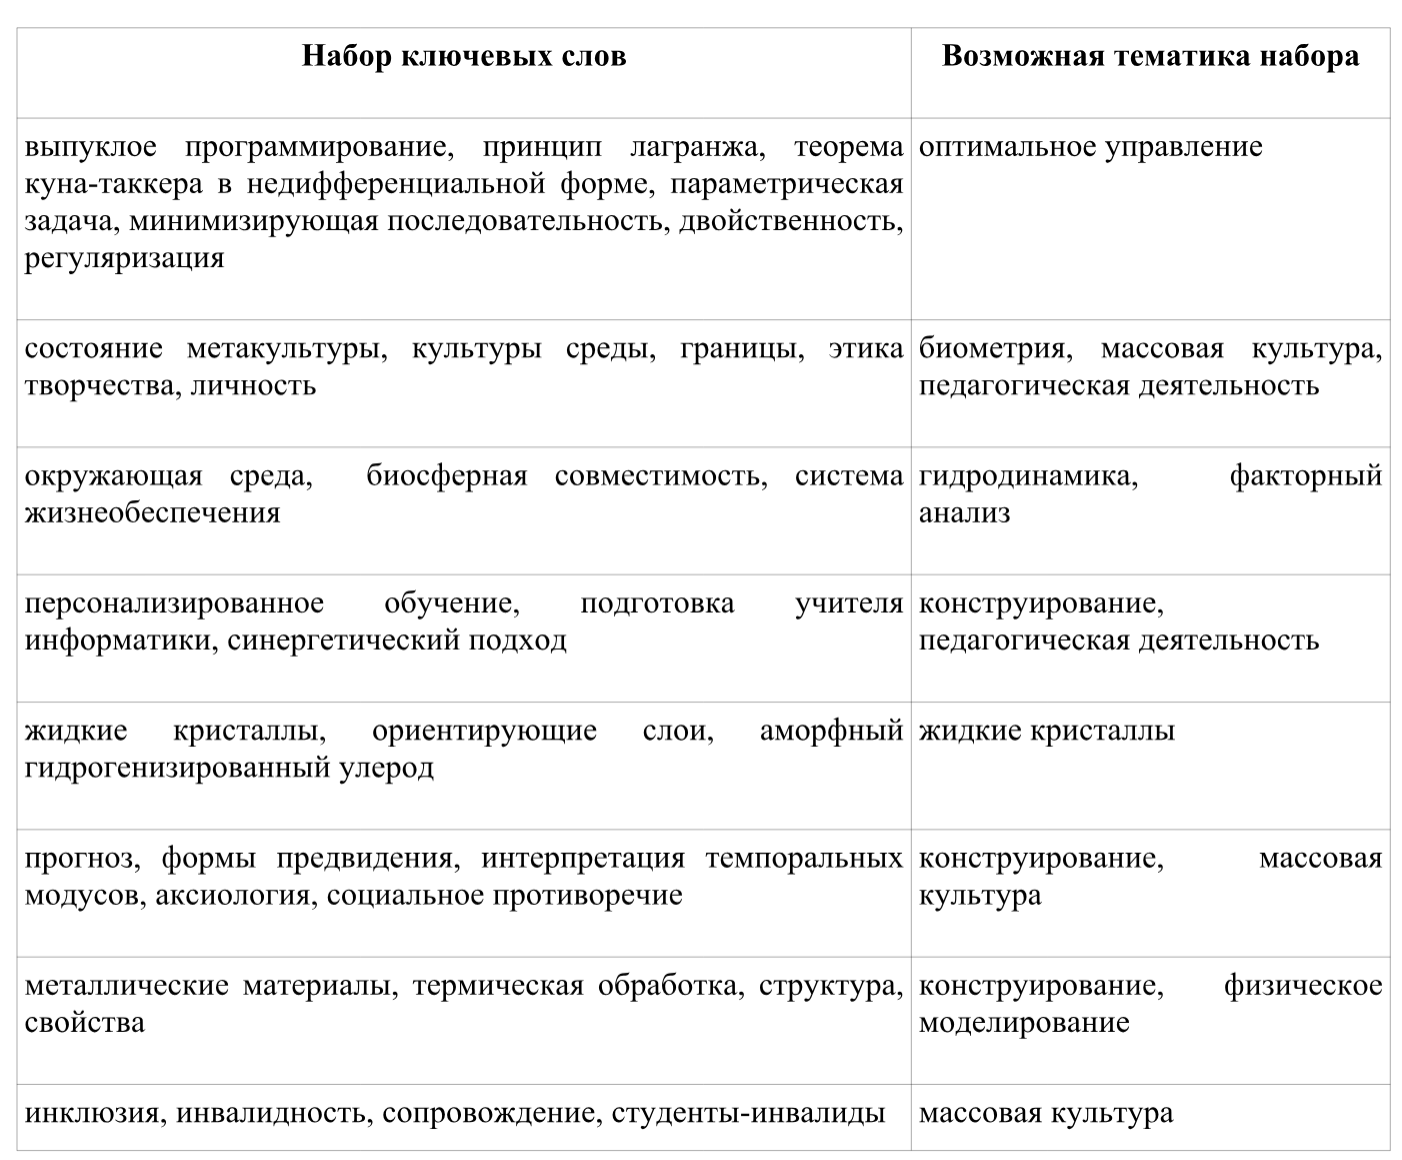
\includegraphics[width=1.0\linewidth]{Dissertation/pics/theme_table_1}
  \end{minipage}
  \label{tbl:theme_table_1}
\end{figure}

\begin{figure}[ht]
  \begin{minipage}[ht]{1.0\linewidth}\centering
    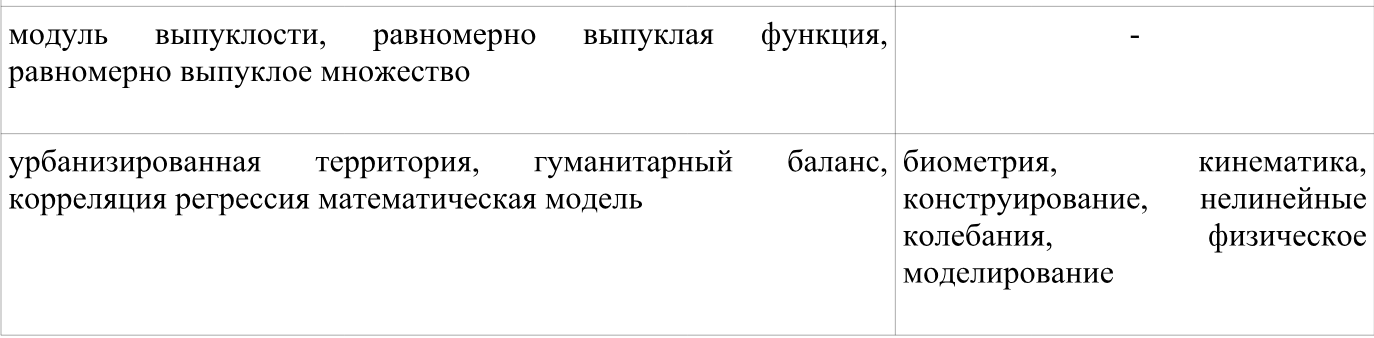
\includegraphics[width=1.0\linewidth]{Dissertation/pics/theme_table_2}
    \caption{Наборы и предсказанные им тематические направления}
  \end{minipage}
  \label{tbl:theme_table_2}
\end{figure}

\hl{В первом примере показано верное определение тематики. При этом можно заметить отсутствие тематического тега в исходном наборе. Последние два примера демонстрируют случаи, когда тематический тег не определён или определено слишком большое число таких тегов.}

\hl{В целом, следует отметить, что алгоритм допускает достаточно много ошибок. Очень часто ошибка возникают на наборах, состоящих только из редких тегов-терминов. Причина в том, что теги в подобных наборах не соединены напрямую с тематическими, а увеличение пути сильно уменьшает качество результатов. Не определяется тематика и у тех наборов, теги которых попали в малые компоненты связности без тематических тегов. Однако основная трудность - это накопление ошибок разных алгоритмов. Сначала тег ошибочно получил высокий уровень абстрактности, затем попал в список тематических и, в итоге, неправильно определил тематику набора. В случае с данными из Веб, ошибка накапливается с этапа сбора данных, поэтому результаты становятся неприемлемо плохими.}

\hl{Несмотря на отмеченные недостатки, предложенный подход потенциально может быть улучшен. Для этого можно использовать все теги из набора для определения тематики, проверять абстрактности вершин на пути от данного тега к тематическому и использовать многие другие эвристики. Это предмет исследования на ближайшее будущее. Однако уже сейчас можно констатировать, что алгоритм способен с некоторой точностью решать поставленную задачу.  }

%\begin{table} [htbp]% Пример записи таблицы с номером, но без отображаемого наименования
%	\centering
%	\parbox{18cm}{% чтобы лучше смотрелось, подбирается самостоятельно
%        \captiondelim{}% должен стоять до самого пустого caption
%        \caption{}%
%        \label{tbl:test1}%
%        \begin{SingleSpace}
%    	\begin{tabular}{ | c | c |}
%    	\hline
%    	выпуклое программирование, принцип лагранжа, \\
%        теорема куна-таккера в недифференциальной форме, \\
%        параметрическая задача, \\
%        минимизирующая последовательность, двойственность\\
%        , регуляризация & оптимальное \\ управление \\ \hline
%    	\end{tabular}%
%    	\end{SingleSpace}
%	}
%\end{table}

\section{Решение задачи поиска экспертов} \label{expert_search_tuplesim}
\subsection{Определение близости наборов для решения задачи поиска экспертов}
В качестве меры близости пары наборов ключевых слов автором предлагается следующая формула:
$$ TupleSim_{expert}(X,Y) = \frac{\sum_{i=1}^{|X|}\sum_{j=1}^{|Y|}WordSim_{expert}(X_i, Y_j)}{|X \bigcup Y|}, $$

где $|\cdot|$ ­ количество слов в наборе, $X_i$, $Y_j$ ­ $i$­ый и $j$­ый теги наборов $X$, $Y$ соответственно. $WordSim_{expert}$ - мера близости, введенная в \ref{expert_search_wordsim}. Числитель этой формулы аккумулирует близость всех пар слов из разных наборов. Если положить $WordSim_{expert}(x, y) = \mathbbm{1}x=y$, то числитель будет равен числу общих тегов, что приведет к более простой модели вычисления близости по мере Жаккара. Без нормировки длинные пары наборов были бы сильнее похожи друг на друга, чем короткие пары.


\section{Тестовые испытания}
...
\section{Выводы}
...
